
% ----------------------------------------------------------------------
%  Set the document class
% ----------------------------------------------------------------------
\documentclass[11pt,a4paper,twoside]{article}

% ----------------------------------------------------------------------
% Define external packages, language, margins, fonts and new commands
% ----------------------------------------------------------------------
%\input{preamble} 
\usepackage[utf8]{inputenc}   % <<<<< Linux
\usepackage[english]{babel} % <<<<< English
\usepackage{notoccite}
\usepackage[skip=0.5\baselineskip]{caption}
\hyphenation{GTKWave}
\usepackage{listings}
\usepackage[all]{nowidow}
\usepackage{amsmath}
\usepackage{indentfirst}
\usepackage{spreadtab}

%blind text
\usepackage{lipsum}

\usepackage{graphicx}
\graphicspath{ {./} {../../figlib/} }
\def\FontLn{% 16 pt normal
  \usefont{T1}{phv}{m}{n}\fontsize{16pt}{16pt}\selectfont}
\def\FontLb{% 16 pt bold
  \usefont{T1}{phv}{b}{n}\fontsize{16pt}{16pt}\selectfont}
\def\FontMn{% 14 pt normal
  \usefont{T1}{phv}{m}{n}\fontsize{14pt}{14pt}\selectfont}
\def\FontMb{% 14 pt bold
  \usefont{T1}{phv}{b}{n}\fontsize{14pt}{14pt}\selectfont}
\def\FontSn{% 12 pt normal
  \usefont{T1}{phv}{m}{n}\fontsize{12pt}{12pt}\selectfont}

% Use Arial font as default
%
\renewcommand{\rmdefault}{phv}
\renewcommand{\sfdefault}{phv}
\usepackage{geometry}	
\geometry{verbose,tmargin=2.5cm,bmargin=2.5cm,lmargin=2.5cm,rmargin=2.5cm}

%\usepackage{setspace}
%\renewcommand{\baselinestretch}{1.5}

\usepackage[pdftex]{hyperref} % enhance documents that are to be
                              % output as HTML and PDF
\hypersetup{colorlinks,       % color text of links and anchors,
                              % eliminates borders around links
%            linkcolor=red,    % color for normal internal links
            linkcolor=black,  % color for normal internal links
            anchorcolor=black,% color for anchor text
%            citecolor=green,  % color for bibliographical citations
            citecolor=black,  % color for bibliographical citations
%            filecolor=magenta,% color for URLs which open local files
            filecolor=black,  % color for URLs which open local files
%            menucolor=red,    % color for Acrobat menu items
            menucolor=black,  % color for Acrobat menu items
%            pagecolor=red,    % color for links to other pages
            pagecolor=black,  % color for links to other pages
%            urlcolor=cyan,    % color for linked URLs
            urlcolor=black,   % color for linked URLs
	          bookmarks=true,         % create PDF bookmarks
	          bookmarksopen=false,    % don't expand bookmarks
	          bookmarksnumbered=true, % number bookmarks
	          pdftitle={report},
            pdfauthor={Ana Azevedo, Artur Gonçalves, Diogo Soares},
%            pdfsubject={Thesis Title},
%            pdfkeywords={Thesis Keywords},
            pdfstartview=FitV,
            pdfdisplaydoctitle=true}

\usepackage[numbers,sort&compress]{natbib} % <<<<< References in numbered list [1],[2],...
\usepackage{subcaption} 
\usepackage{mdframed}

%%%%%%%%%%%%%%%%%%%%%%%%%%%%%%%%%%%%%%%%%%%%%%%%%%%%%%%%%%%%%%%%%%%%%%%%
%     Begin Document                                                   %
%%%%%%%%%%%%%%%%%%%%%%%%%%%%%%%%%%%%%%%%%%%%%%%%%%%%%%%%%%%%%%%%%%%%%%%%


\begin{document}

% Set plain page style (no headers, footer with centered page number)
\pagestyle{plain}

% Set roman numbering (i,ii,...) before the start of chapters
%\pagenumbering{roman}

% ----------------------------------------------------------------------
%  Cover page
% ----------------------------------------------------------------------
%%%%%%%%%%%%%%%%%%%%%%%%%%%%%%%%%%%%%%%%%%%%%%%%%%%%%%%%%%%%%%%%%%%%%%%%
%                                                                      %
%     File: Thesis_FrontCover.tex                                      %
%     Tex Master: Thesis.tex                                           %
%                                                                      %
%     Author: Andre C. Marta                                           %
%     Last modified :  2 Jul 2015                                      %
%                                                                      %
%%%%%%%%%%%%%%%%%%%%%%%%%%%%%%%%%%%%%%%%%%%%%%%%%%%%%%%%%%%%%%%%%%%%%%%%

\thispagestyle {empty}

% IST Logo - Signature A
% parameters: bb=llx lly urx ury (bounding box), width=h_length, height=v_length, angle=angle, scale=factor, clip=true/false, draft=true/false. 
\includegraphics[bb=9.5cm 11cm 0cm 0cm,scale=0.29]{IST_A_CMYK_POS}

\begin{center}
%
% Figure (Image or plot)
\vspace{1.0cm}
% height = 50 mm
%\includegraphics[height=50mm]{Figures/Airbus_A350.jpg}

% Title, author and degree
\vspace{3cm}
\textsc{\Huge Lab 1: Circuit analysis methods}\\
\vspace{0.5cm}
{\Large Circuit Theory and Electronics Fundamentals} \\
\vspace{0.8cm}
{\normalsize Ana Bárbara Azevedo (96504), Artur Gonçalves (96513), Diogo Soares (96519)} \\

\vspace{0.5cm}
{March 23, 2021}\\
\end{center}
\vspace{2.5cm}



% ----------------------------------------------------------------------
% Dedication page (optional)
% ----------------------------------------------------------------------
%\input{dedication} 
%\cleardoublepage

% ----------------------------------------------------------------------
%  Acknowledgments (optional)
% ----------------------------------------------------------------------
%\input{acknowledgements}
%\cleardoublepage

% ----------------------------------------------------------------------
%  Abstract (both in English and Portuguese)
% ----------------------------------------------------------------------
%\input{resumo} 
%\cleardoublepage

%\input{abstract} 

% ----------------------------------------------------------------------
%  Table of contents, list of tables, list of figures and nomenclature
% ----------------------------------------------------------------------

% Table of contents
%
\tableofcontents

% List of tables
%\addcontentsline{toc}{section}{\listtablename}
%\listoftables
%\cleardoublepage 

% List of figures
%\addcontentsline{toc}{section}{\listfigurename}
%\listoffigures
%\cleardoublepage 

% Set arabic numbering (1,2,...) after preface
%
%\setcounter{page}{1}
%\pagenumbering{arabic}

% ----------------------------------------------------------------------
%  Body
% ----------------------------------------------------------------------

\newpage
\section{Introduction}
\label{sec:introduction}

% state the learning objective 
\par In this laboratory assignment, a circuit containing both an independent (first constant and then sinusoidal) and a current controlled voltage sources ($V_s$ and $V_d$, respectively), a voltage controlled current source ($I_b$), connected to multiple resistors (from $R_{1}$ to $R_{7}$) and a capacitor ($C$) is going to be studied. The described circuit can be observed in detail in Figure~\ref{fig:rc}.

\par In Section~\ref{sec:theoretical}, a theoretical analysis of the circuit is presented, studying the static, time and frequency responses, using the Octave tool. After that, in Section~\ref{sec:simulation}, the circuit is analysed via simulation, using the software Ngspice. The obtained results are then compared, explaining the reasons behind the differences and similarities found. Finally, one can find the conclusions of this study outlined in Section~\ref{sec:conclusion}.

\begin{figure}[h] \centering
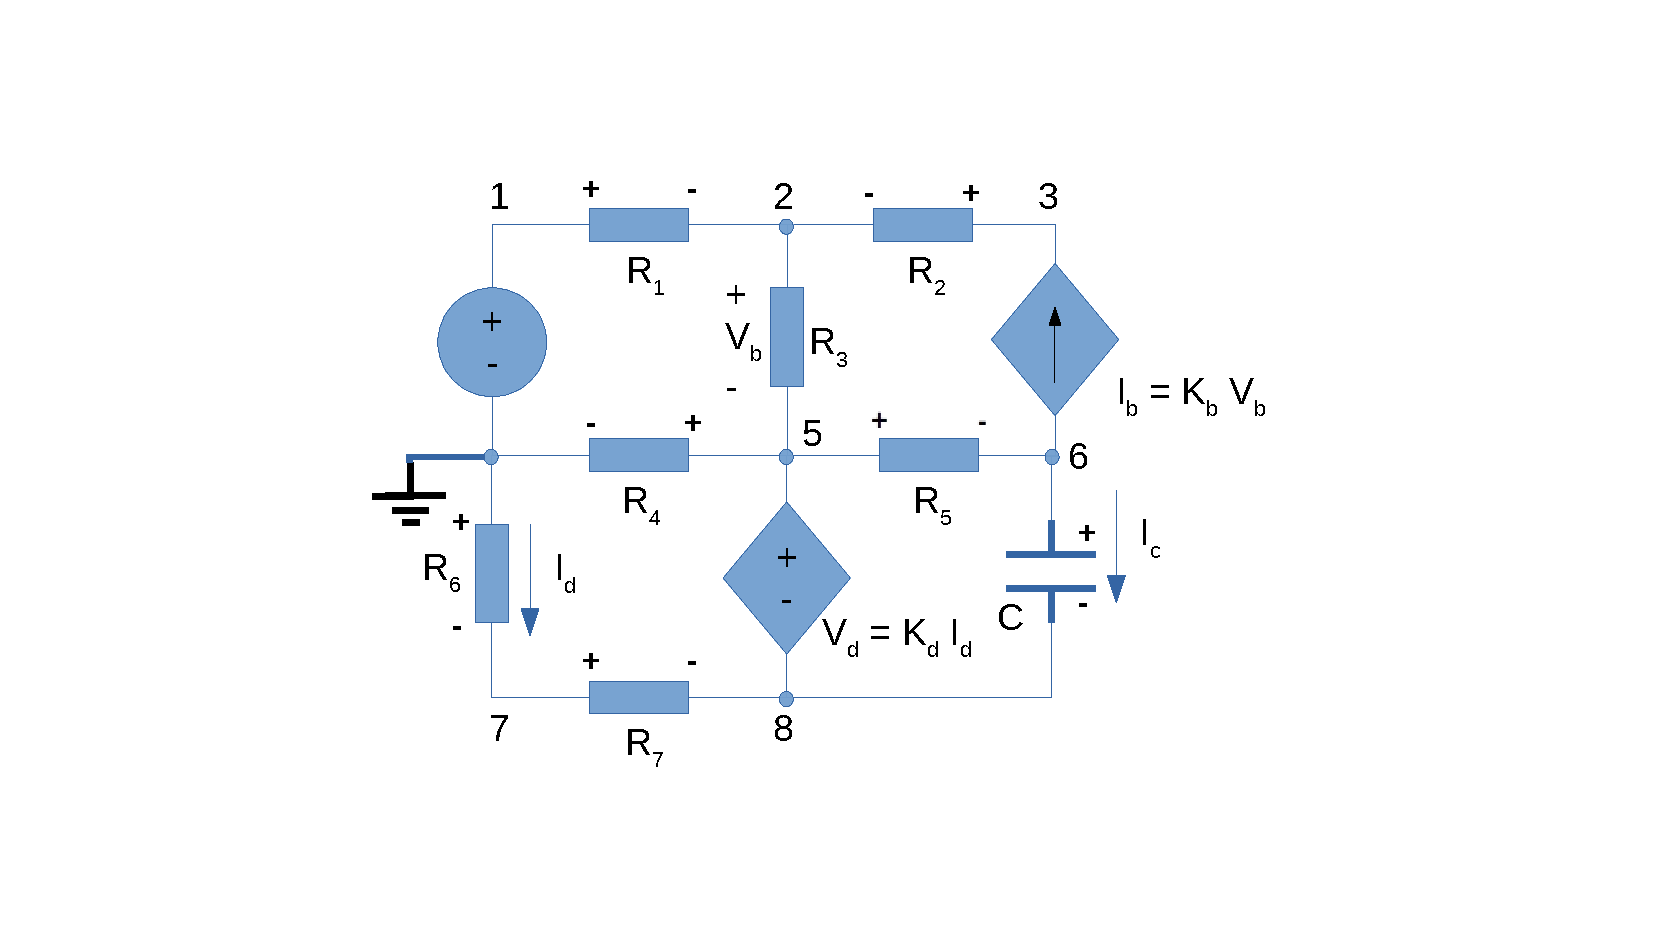
\includegraphics[width=1.1\linewidth]{rc.pdf}
\caption{Circuit diagram.}
\label{fig:rc}
\end{figure}


\section{Theoretical Analysis}
\label{sec:theoretical}
\vspace{3mm}
In this section, the previously shown circuit is theoretically analised. It is important to remember that its behaviour depends on the consideration of two different time intervals, as $v_s(t)$ is defined as a piecewise function:
\vspace{3mm}


\begin{center}
$v_s(t) =\begin{cases} V_s \quad \quad \quad \quad ,t<0\\ sin(2\pi ft) \quad ,t \geq 0 \end{cases}$
\vspace{5mm}
\end{center}

\vspace{3mm}

\subsection{Nodal Analysis for $t<0$} \label{teo:2.1}
\vspace{3mm}

\par For $t<0$, $v_s(t)$ assumes a constant value $V_s$ for excitation. Besides that, the system has had enough time for it to overcome any transitional period, which means all the electric quantities in the circuit have had the time to stabilize, and so the current that passes through the capacitor $i_c(t)$ is null, because $i_c(t)=C\frac{dv_c(t)}{dt}$ and $\frac{dv_c(t)}{dt}=0$ (since $v_c(t)$ is no longer varying). Therefore, we can consider an open circuit as a replacement for the capacitor branch.

\vspace{3mm}
\par In order to determine the voltages in all nodes and, hence, the currents in all branches, nodal analysis is applied to the circuit, as suggested by the following system:

\begin{center}
  $\begin{cases} V_1=V_s  \\ (V_2-V_1)G_1 + (V_2-V_3)G_2 + (V_2-V_5)G_3=0 \\ (V_3-V_2)G_2 - K_b(V_2-V_5)=0 \\ (V_5-V_2)G_3 + (V_5-V_6)G_5 + V_5G_4 + (V_8-V_7)G_7 =0 \\ K_b(V_2-V_5)+(V_6-V_5)G_5=0 \\ (V_7-V_8)G_7 + V_7G_6 =0 \\ V_8-V_5 - K_dV_7G_6=0 \end{cases}$
\end{center}

Note that some substitutions were made, such as:

\vspace{3mm}
\begin{equation}
  \label{eq4}
   I_b = K_b(V_2-V_5)
\end{equation}
\begin{equation}
  \label{eq5}
   V_d=-K_dV_7G_6
\end{equation}
\vspace{3mm}


\par By solving this system using Octave, the voltages that follow are obtained for every node. On the other hand, defining branch currents accordingly to the conventional electric current flow (from the plus to the minus sign defined in the figure), one obtains the subsequent values for each branch (using Ohm's law). For the sake of direct comparison, the results that follow the simulation analysis are already shown in this segment as well.

\renewcommand{\arraystretch}{1.5}
\begin{table}[htbp]
\begin{minipage}{.3\textwidth}
\centering

\begin{tabular}{|c|c|}
\hline    
\textbf{Variable name} & \textbf{Value [A or V]} \\ \hline
$I_b$ & -2.540344e-04\\ \hline
$I_{R_1}$ & 2.428274e-04\\ \hline
$I_{R_2}$ & -2.540344e-04\\ \hline
$I_{R_3}$ & -1.120696e-05\\ \hline
$I_{R_4}$ & 1.176699e-03\\ \hline
$I_{R_5}$ & -2.540344e-04\\ \hline
$I_{R_6}$ & 9.338720e-04\\ \hline
$I_{R_7}$ & 9.338720e-04\\ \hline
$V_1$ & 5.046144e+00\\ \hline
$V_2$ & 4.802884e+00\\ \hline
$V_3$ & 4.276252e+00\\ \hline
$V_5$ & 4.837826e+00\\ \hline
$V_6$ & 5.626501e+00\\ \hline 
$V_7$ & -1.934734e+00\\ \hline 
$V_8$ & -2.909165e+00\\ \hline 
$I_s$ & -2.428274e-04\\ \hline 
$I_d$ & -9.338720e-04\\ \hline

\end{tabular}
\end{minipage}
\hspace{50px}
\begin {minipage}{.8\textwidth}
\centering

\begin{tabular}{|c|c|}
\hline    
\textbf{Variable name} & \textbf{Value [A or V]} \\ \hline
ymax & 1.199966e+01\\ \hline
ymin & 1.199965e+01\\ \hline
yavg & 1.199966e+01\\ \hline
ripple & 1.000000e-05\\ \hline
merit & -2.52956e+00\\ \hline

\end{tabular}
\end{minipage}
\caption{On the left, nodal analysis and current values for $t<0$ by Octave. On the right, operating point analysis for $t<0$ by Ngspice: a variable preceded by @ is of type \textit{current} and expressed in Ampere; other variables are of type \textit {voltage} and expressed in Volt. $gb$ refers to the controlled current source $I_b$ and the rest is defined as before. \small Notes: $v_4$ refers to a special added node, which will be explained on \ref{sec:simulation}; the 2 last values on the left table cannot be directly seen on the right table, but can be easily deduced from the ones presented.}
\label{tab_1}
\end{table}



\newpage
\subsection{Nodal analysis for $t=0$, equivalent Resistance $R_{eq}$, Time Constant $\tau$} \label{teo:2.2}


\vspace{3mm}
\par Making $V_s=0$ (node 1 also becomes GND), the $t=0$ voltage levels for each node can be calculated, by also replacing the capacitor with a voltage source $V_x=V_6-V_8$, with $V_6$ and $V_8$ being the voltages in \ref{tab_1}. This can be done because $V_6-V_8$ remains the same for $t<0$ and $t=0$ (because the capacitor does not discharge instantly). The new circuit is, again, analysed with the Nodal Method, as suggested by the following system (results on table \ref{zdsca}):


\begin{center}
  $\begin{cases} V_2G_1 + (V_2-V_3)G_2 + (V_2-V_5)G_3=0 \\ -K_b(V_2-V_5)+(V_3-V_2)G_2=0 \\ V_5G_4 + (V_5-V_6)G_5 + (V_5-V_2)G_3 + (V_8-V_7)G_7 - [-K_b(V_2-V_5) + (V_5-V_6)G_5] =0 \\ V_6-V_8=V_x \\ V_7G_6+(V_7-V_8)G_7=0 \\ V_8-V_5 - K_dV_7G_6=0 \end{cases}$
\end{center}


\par Again, some substitutions were made, such as:

\vspace{3mm}
\begin{equation}
  \label{a}
   I_b = K_b(V_2-V_5)
\end{equation}
\begin{equation}
  \label{aa}
   V_d=-K_dV_7G_6
\end{equation}
\begin{equation}
  \label{aaa}
   I_x = -I_b + (V_5-V_6)G_5
\end{equation}
\vspace{3mm}

with $I_x$ being the current that flows downwards in $V_x$ (positive sign up in $V_x$).

\vspace{3mm}
\par This circuit can be seen as a simple RC circuit, with the voltage source $V_x$ and the current that flows in the mesh being $I_x=-K_b(V_2-V_5) + (V_5-V_6)G_5$. Of course, all the remaining circuit, as seen by the capacitor's terminals, works as an equivalent resistor. Its equivalent resistance can be calculated with the expression

\begin{equation}
  R_{eq}=-\frac{V_x}{I_x}
\end{equation}

with $R_{eq}$ being the equivalent resistance as seen by the capacitor's terminals.

\vspace{3mm}
\par The minus sign results from the fact that, in the equivalent circuit, $I_x$ flows through the equivalent resistor from the negative to the positive terminal (in opposition to the convention).
Thus, the time constant for the equivalent circuit $\tau$  can be computed as $R_{eq}C$.

\vspace{3mm}
\par By solving the refered system using Octave, the following table presents the voltage in every node, as well as the equivalent resistance and the time constant (once again, one can imediately consult the simulation values as well).



\renewcommand{\arraystretch}{1.5}
\begin{table}[htbp]
\begin{minipage}{.3\textwidth}
\centering

\begin{tabular}{|c|c|}
\hline    
\textbf{Variable name} & \textbf{Value [A or V or $\Omega$]} \\ \hline
$I_b$ & -0.000000e+00\\ \hline
$I_{R_1}$ & 0.000000e+00\\ \hline
$I_{R_2}$ & 0.000000e+00\\ \hline
$I_{R_3}$ & -0.000000e+00\\ \hline
$I_{R_4}$ & 0.000000e+00\\ \hline
$I_{R_5}$ & -2.749362e-03\\ \hline
$I_{R_6}$ & 0.000000e+00\\ \hline
$I_{R_7}$ & 0.000000e+00\\ \hline
$V_2$ & -0.000000e+00\\ \hline
$V_3$ & 0.000000e+00\\ \hline
$V_5$ & 0.000000e+00\\ \hline
$V_6$ & 8.535665e+00\\ \hline 
$V_7$ & -0.000000e+00\\ \hline 
$V_8$ & -0.000000e+00\\ \hline 
$I_x$ & -2.749362e-03\\ \hline 
$R_{eq}$ & 3.104598e+03\\ \hline
$\tau$ & 3.224319e-03\\ \hline

\end{tabular}
\end{minipage}
\hspace{50px}
\begin {minipage}{.8\textwidth}
\centering

\begin{tabular}{|c|c|}
\hline    
\textbf{Variable name} & \textbf{Value [A or V]} \\ \hline
@gb[i] & 0.000000e+00\\ \hline
@r1[i] & 0.000000e+00\\ \hline
@r2[i] & 0.000000e+00\\ \hline
@r3[i] & 0.000000e+00\\ \hline
@r4[i] & 0.000000e+00\\ \hline
@r5[i] & -2.74936e-03\\ \hline
@r6[i] & 0.000000e+00\\ \hline
@r7[i] & 0.000000e+00\\ \hline
v(2) & 0.000000e+00\\ \hline
v(3) & 0.000000e+00\\ \hline
v(4) & 0.000000e+00\\ \hline
v(5) & 0.000000e+00\\ \hline
v(6) & 8.535665e+00\\ \hline
v(7) & 0.000000e+00\\ \hline
v(8) & 0.000000e+00\\ \hline

\end{tabular}
\end{minipage}
\caption{On the left, nodal analysis, current values, equivalent resistance and time constant for $t=0$ and $v_s(t)=0$ by Octave. On the right, operating point analysis for $t=0$ by Ngspice: a variable preceded by @ is of type \textit{current} and expressed in Ampere; other variables are of type \textit {voltage} and expressed in Volt. $gb$ refers to the controlled current source $I_b$ and the rest is defined as before. \small Notes: $v_4$ refers to a special added node, which will be explained on \ref{sec:simulation}; the 2 last values on the left table cannot be directly seen on the right table, but can be easily deduced from the ones presented.}
\label{tab_2}
\end{table}


\newpage

\subsection{Natural Solution $v_{6n}(t)$}

\vspace{3mm}
\par Let's consider the situation for $t\geq0$. The circuit's solution can be described as the superposition of two components. The natural solution, which is the system's behaviour with no external excitation (it leads to the capacitor's discharge), and the forced solution, which will allow an oscillating steady-state.

\vspace{3mm}
\par To compute the natural solution, particularly, for node $6$ ($v_{6n}$), the circuit is considered to be the previously refered simple RC circuit with the capacitor $C$ and the equivalent resistor $R_{eq}$.
The following deduction applies KVL to the mesh, uses the capacitor's law to replace the mesh's current ($i_c(t)=C\frac{dv_c(t)}{dt}$), and solves the resulting differential equation:

\begin{equation}
 v_c+R_{eq}i=0 \Leftrightarrow v_c+R_{eq}C\frac{dv_c}{dt}=0 \Leftrightarrow v_c(t)=Ae^{-\frac{t}{R_{eq}C}}=
\end{equation}

\par The constant $A$ is determined by the initial condition as being the capacitor's voltage $v_c(0)=V_x=V_6-V_8$ at $t<0$. Considering the values obtained in the previous section for voltages in \ref{tab_2}, the natural solution for $V_6$ becomes

\begin{equation}
  v_{6n}(t)=V_xe^{-\frac{t}{R_{eq}C}}=8.53567e^{-\frac{t}{0.22432 \times 10^{-3}}} [V]
\end{equation}

\par The following figure represents its plot in the interval $[0,20]$ms:

\begin{figure}[h]
     \centering
         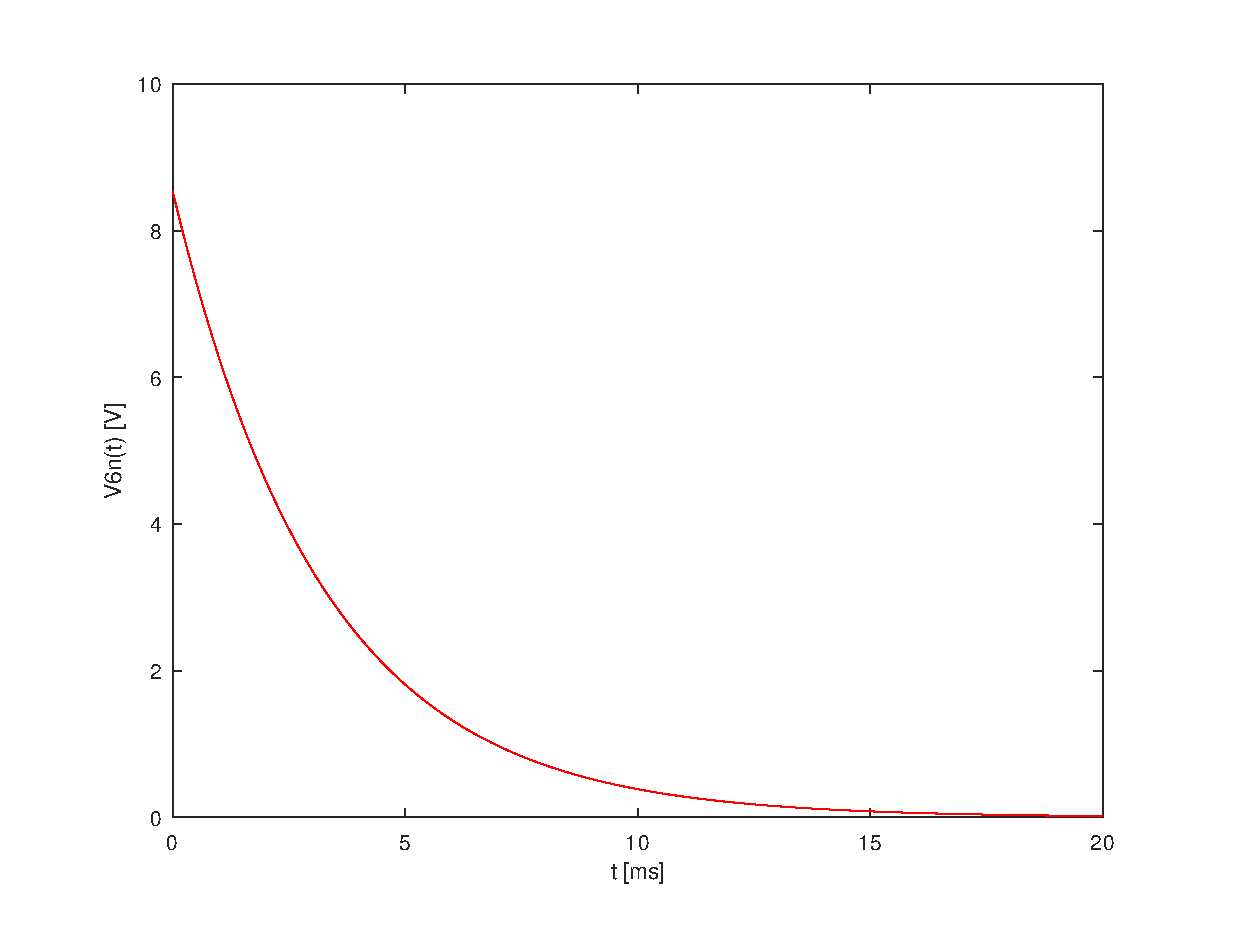
\includegraphics[scale = 0.7]{v6n.eps}
         \caption{$v_{6n}(t)$ in the interval $[0, 20]$ $ms$.}
     \label{v6n}
 \end{figure}
 \vspace{5mm}


\subsection{Forced Solution $v_{6f}(t)$}
In order to compute the forced solution for $t\geq0$, consequence of the sinusoidal excitacion due to the source $V_1$, in $t\geq0$, it is considered the frequency $f=1$kHz and a phasor voltage $\widetilde{V_s}=1$. The circuit in figure \ref{fig:rc} is analysed using the Nodal Method (applied to phasors), as suggested by the following system, with $Y_x$ being the admittances of the components ($G_x$ for resistors and $2\pi fCj$ for the capacitor)


\begin{center}
  $\begin{cases} \widetilde{V_1}= \widetilde{V_s} \\ (\widetilde{V_2}-\widetilde{V_1})Y_1 + (\widetilde{V_2}-\widetilde{V_3})Y_2 + (\widetilde{V_2}-\widetilde{V_5})Y_3=0 \\  (\widetilde{V_3}-\widetilde{V_2})Y_2 -K_b(\widetilde{V_2}-\widetilde{V_5})=0 \\ (\widetilde{V_5}-\widetilde{V_2})Y_3 + \widetilde{V_5}Y_4 + (\widetilde{V_5}-\widetilde{V_6})Y_5 + (\widetilde{V_8}-\widetilde{V_7})Y_7 + (\widetilde{V_8}-\widetilde{V_6})Y_C=0 \\ (\widetilde{V_6}-\widetilde{V_5})Y_5 + (\widetilde{V_6}-\widetilde{V_8})Y_C + K_b(\widetilde{V_2}-\widetilde{V_5})=0 \\ \widetilde{V_7}Y_6 + (\widetilde{V_7}-\widetilde{V_8})Y_7 =0 \\ (\widetilde{V_8}-\widetilde{V_5}) - K_d\widetilde{V_7}Y_6=0 \end{cases}$
\end{center}

Note that, once again, some substitutions were made, such as:

\vspace{3mm}
\begin{equation}
  \label{eq5}
   \widetilde{I_b} = K_b(\widetilde{V_2}-\widetilde{V_5})
\end{equation}
\begin{equation}
  \label{eq6}
   \widetilde{V_d}=-K_d\widetilde{V_7}Y_6
\end{equation}
\vspace{3mm}

\par By solving the system using Octave, the following table presents the complex amplitude (phasor) in every node:

\renewcommand{\arraystretch}{1.5}
\begin{table}[h]
  \centering
  \begin{tabular}{|c|c|}
    \hline    
    \textbf{Complex amplitude} & \textbf{Value} \\ \hline
    $\widetilde{V_1}$ & 1.000000+0.000000j\\ \hline
$\widetilde{V_2}$ & 0.951793-0.000000j\\ \hline
$\widetilde{V_3}$ & 0.847430-0.000000j\\ \hline
$\widetilde{V_5}$ & 0.958717-0.000000j\\ \hline
$\widetilde{V_6}$ & -0.572401-0.083292j\\ \hline
$\widetilde{V_7}$ & -0.383408+0.000000j\\ \hline
$\widetilde{V_8}$ & -0.576512+0.000000j\\ \hline

  \end{tabular}
  \caption{Complex amplitude values for every node (forced solution, $t\geq0$.}
  \label{tab_3}
\end{table}

\par The expression for the real forced solution in $\widetilde{V_6}$ can be calculated the following way (considering $\widetilde{V_1}=1$):

\vspace{3mm}
\begin{equation}
  \label{eq7}
   \frac{\widetilde{V_6}}{\widetilde{V_1}} = a + jb=|a + jb|e^{-j(-\phi)},\quad a,b \in \mathbb{R},\quad \phi \quad \textrm{the angle of} \quad  a + jb
\end{equation}

\par One then has:

\vspace{3mm}
\begin{equation}
  \label{eq8}
   \frac{V_6}{V_1} = |a + jb|
\end{equation}

\begin{equation}
  \label{eq9}
   \phi_6-\phi_1=\phi
\end{equation}

\par Using the values of table \ref{tab_3}, one obtains:

\begin{equation}
  \label{eq10}
   v_{6f}(t)=0.57843\sin(2\pi \times 1000t - 2.9971) [V]
\end{equation}

\par Note that this process is usually made when the input voltage source is in the form of a cosine. By doing some algebraic manipulation, one can come to the conclusion that the use of sines is totally analogue.

\vspace{5mm}
\subsection{Total Solution $v_6(t)$}

\vspace{5mm}
\par As previously said, the total solution consists on the superposition of both natural and forced solutions. Hence,

\begin{equation}
v_6(t)=v_{6n}(t)+v_{6f}(t)=8.53567e^{-\frac{t}{0.22432 \times 10^{-3}}}+0.57843\sin(2\pi \times 1000t - 2.9971) [V]
\end{equation}

\vspace{3mm}
\par The following figure represents the plot of both $v_s(t)$ and $v_6(t)$, in the interval $[-5,20]$ms. Note that this time range includes the transition at $t=0$. Therefore, it is normal to observe a discontinuity at $t=0$, from the constant to the oscillating solution.


\begin{figure}[h]
     \centering
         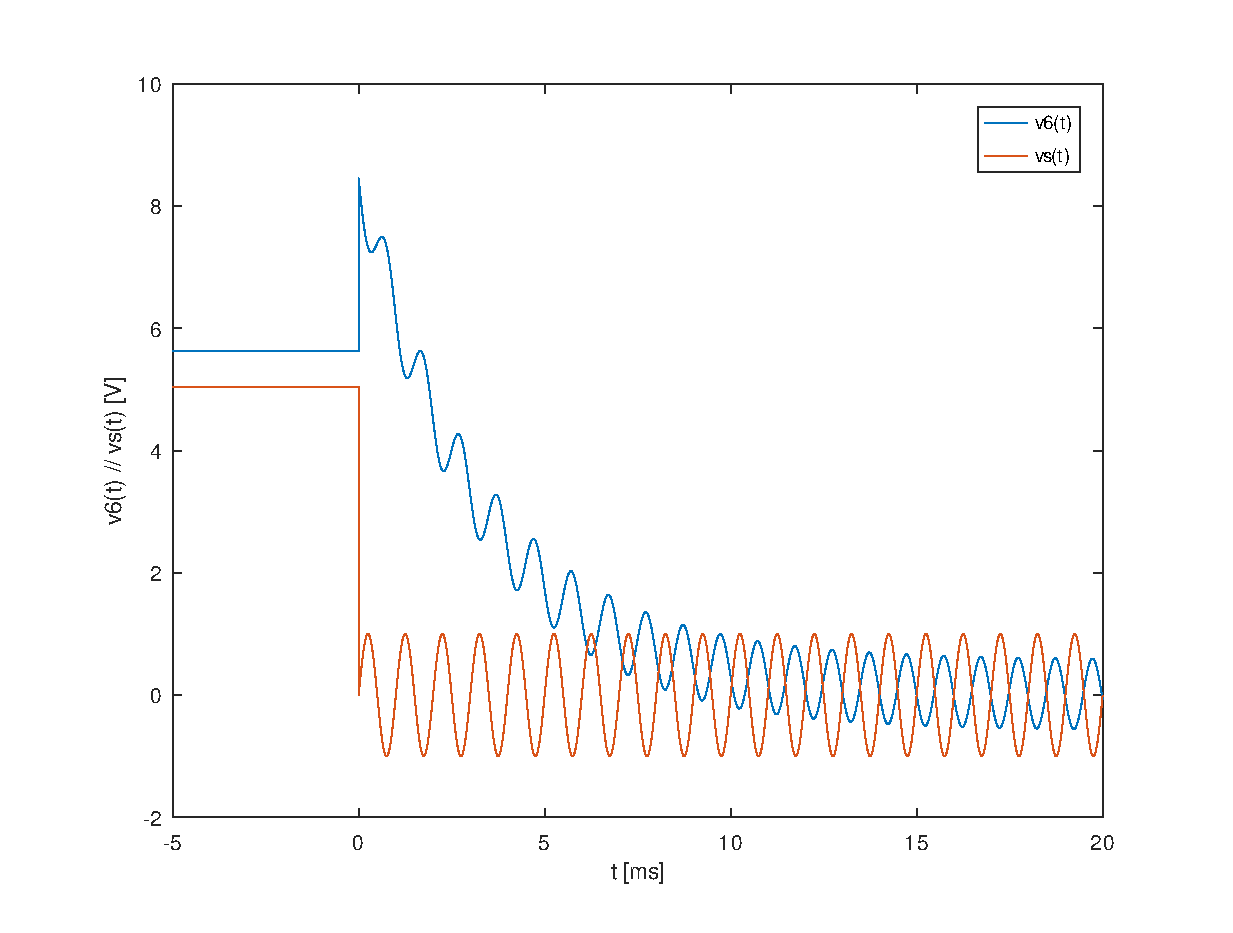
\includegraphics[scale = 0.7]{v6t.eps}
         \caption{$v_s(t)$ and $v_{6}(t)$ in the interval $[-5, 20]$ $ms$.}
     \label{v6t}
 \end{figure}
 \vspace{5mm}


\vspace{3mm}
\par It can be observed the effect of the dissipative solution (natural), which leads to a voltage decrease, until it vanishes, only remaining the forced solution, which shows a steady-state harmonic oscillation.


\vspace{+5mm}


\vspace{5mm}
\subsection{Frequency analysis} \label{teo:2.6}

\par It is possible to study the effect of the input ($v_s(t)$) frequency $f$ in the output signal $v_c(t)=v_6(t)-v_8(t)$ or in any of the system nodes. This way, it is displayed the plot for both the magnitude in dB (Figure \ref{abs_v6vcvs}) and phase in degrees (Figure \ref{phase_v6vcvs}) of the signals $v_c$ and $v_6$ as function of $f$ and also of $v_s$ (for comparison). The type of scale chosen for the frequency axis $-$ logscale $-$ is convenient to make big plot ranges fit in small figures.

\begin{figure}[h]
     \centering
         \includegraphics[scale = 0.55]{abs_v6vcvs.eps}
         \caption{Magnitude of $v_s$ and magnitude responses of $v_{6}$ and $v_{c}$.}
     \label{abs_v6vcvs}
 \end{figure}
 \vspace{5mm}

\par An RC circuit behaves like a low-pass filter (blocks high frequencies and passes low frequencies). That is, at low frequencies, there's a very small magnitude response of the output frequency $v_c$. One can look at the plot and see that, for values of $f$ close to $0$, $v_c$ and $v_6$ both have an amplitude of approximately $0$ $dB$, which translates to $1V$ (the same as $v_{s}$ $-$ no response).
\par On the other side, for high frequencies (as soon as it reaches cut-off frequency $\approx -3dB$), the magnitude (dB) of the output becomes more and more negative, with a slope of $-20dB/decade$ (this values can be obtained through the system's transfer function). This means the output voltage value in volt becomes lower and lower (high signal attenuation). The impedance of a capacitor decreases with as the input frequency increases, which means it will each time offers less resistance to the current flow between its terminals, so one can almost decribe it as a short-circuit (zero output).

\vspace{3mm}
\par Keep in mind that the circuit does not have any amplifying elements (\textit{e.g.}, transistors), so the output level is almost always less/equal to the input one. 

\newpage
 \begin{figure}[h]
     \centering
         \includegraphics[scale = 0.55]{phase_v6vcvs.eps}
         \caption{Phase of $v_{s}$ and phase responses of $v_{6}$ and $v_{c}$.}
     \label{phase_v6vcvs}
 \end{figure}
 \vspace{5mm}

 \par As it can be seen, for high frequencies (from about $10^3 Hz$), the voltage value registered in node 6 presents a phase close to $-\pi$, which means it is in phase opposition with the input voltage source $v_s$. That can be easily confirmed by the observation of Figure \ref{v6t}, in which the plot is made precisely for $1$ $KHz$. Considering $v_c$, it lags behind the source as well (in $\pi/2$). This happens because the excitation is changing too fast for the output to be able to keep up with it (it takes time to charge the capacitor's plates while the input voltage is changing). The sudden drop happens for two decades, arround the time $\omega=2\pi f$ achieves the value of $\frac{1}{R_{eq}C}$ (which is analogue to the ressonance/natural frequency of a spring-mass system). That would be pretty evident, once again, by looking at the transfer function for the equivalent circuit previously described (which, in this case, represents the value of $\widetilde{V_c}$, since $\widetilde{V_s}=1$). Its angle is given by $-\arctan(\omega R_{eq}C)$, so for $\omega =\frac{1}{R_{eq}C}$ we get a value of $-\frac{\pi}{4}$, which is the central value of the phase drop of $v_{c}$.




\section{Simulation Analysis}
\label{sec:simulation}
\captionsetup[table]{skip=10pt}

\subsection{Operating Point Analysis}

\vspace{5mm}
\par Table \ref{tab_op} shows the simulated operating point results (obtained from Ngspice) for the circuit under analysis, considering that current directions $I_1$, $I_2$, $I_3$ and $I_4$ (and, accordingly, the positive and negative terminals of the components) were defined based on the same model as before.


\renewcommand{\arraystretch}{1.5}
\begin{table}[h]
  \centering
  \begin{tabular}{|c|c|}
    \hline    
    \textbf{Variable name} & \textbf{Value [mA or V]} \\ \hline
    @gb[i] & -2.00589e-01\\ \hline
@id[current] & 1.017967e+00\\ \hline
@r1[i] & 1.915709e-01\\ \hline
@r2[i] & -2.00589e-01\\ \hline
@r3[i] & -9.01783e-03\\ \hline
@r4[i] & 1.164729e+00\\ \hline
@r5[i] & -1.21856e+00\\ \hline
@r6[i] & 9.731579e-01\\ \hline
@r7[i] & 9.731579e-01\\ \hline
v(1) & 8.030092e+00\\ \hline
v(2) & 7.833907e+00\\ \hline
v(3) & 7.417135e+00\\ \hline
v(4) & 2.989101e+00\\ \hline
v(5) & 7.861734e+00\\ \hline
v(6) & 1.163284e+01\\ \hline
v(7) & 9.951293e-01\\ \hline
v(8) & 2.989101e+00\\ \hline

  \end{tabular}
  \caption{Operating point analysis - a variable preceded by @ is of type \textit{current} and expressed in miliAmpere; other variables are of type \textit {voltage} and expressed in Volt. $gb$ refers to the controlled current source $I_b$ and the rest is defined as before.}
  \label{tab_op}
\end{table}
\vspace{3mm}
\par Compared to the theoretical analysis results, one notices a few differences.
\vspace{3mm}
\par Focusing on the obtained nodal voltage levels, an almost exact resemblance is shown, except for the fact that Octave's used result precision is of 6 decimal places, whereas Ngspice always presents 7 significant digits (hence the small differences). It's worth noting that node 8 (introduced exclusively on the simulation analysis) was created so a zero valued voltage source (working as an ammeter) could be placed in series with resistor 6, allowing the algorithm to measure the current between nodes 4 and 7.
\vspace{3mm}
\par The same issue takes place with the current values, altough we can only directly compare four of them: $I_1$ with $@r2[i]$, $I_2$ with $@r1[i]$, $I_3$ with both $@r6[i]$ and $@r7[i]$ as well as $I_4$ with the symmetric of $I_d$, as stated on section \ref{sec:analysis} (even if it was rather an input value and not quite an output one). For further comparisons, proceed as indicated in sections \ref{sec:2.1} and \ref{sec:2.2}.
\vspace{3mm}
\par Other than that, we could say there's a perfect match on the results obtained from both analysis methods.
\vspace{5mm}







\section{Conclusion}
\label{sec:conclusion}
\vspace{3mm}
\par In this laboratory assignment, the goal of analysing the circuit has been achieved. Theoretically, both node and mesh analyses have been performed, and the results were obtained using the Octave maths tool. Besides that, a circuit simulation, using the Ngspice tool, was also executed. The simulation results matched the theoretical results almost precisely, as explained in Section~\ref{sec:simulation}. The excellent match relies on the fact that this is a quite straightforward circuit, containing only linear and simple components. So, eventhough the theoretical and simulation models could differ - when using more complex components- this is not the case in this work.
\vspace{3mm}
\par In conclusion, we confirmed that this was a very important circuit to study, since it allowed us to expand our understanding of the basics of electronic circuits. It was also pretty curious for us to apply some physics concepts we have learned in other disciplines when studying this circuit and being able to testify that they work in practise.

%\cleardoublepage

% ----------------------------------------------------------------------
%  Bibliography
% ----------------------------------------------------------------------
%\addcontentsline{toc}{section}{\bibname}
%\bibliographystyle{abbrvunsrtnat} % <<<<< SELECT IF USING REFERENCES BY NUMBER (CITATION ORDER)
%\bibliography{../../../BIBfile.bib}

% ----------------------------------------------------------------------
\end{document}
% ----------------------------------------------------------------------

